\documentclass{article} % For LaTeX2e
\usepackage{iclr2022_conference,times}
\usepackage{tabularx}
\usepackage{array}
\usepackage{caption}
\usepackage{booktabs}
\usepackage[table]{xcolor}
\usepackage{makecell}
% Optional math commands from https://github.com/goodfeli/dlbook_notation.
%%%%% NEW MATH DEFINITIONS %%%%%

\usepackage{amsmath,amsfonts,bm}

% Mark sections of captions for referring to divisions of figures
\newcommand{\figleft}{{\em (Left)}}
\newcommand{\figcenter}{{\em (Center)}}
\newcommand{\figright}{{\em (Right)}}
\newcommand{\figtop}{{\em (Top)}}
\newcommand{\figbottom}{{\em (Bottom)}}
\newcommand{\captiona}{{\em (a)}}
\newcommand{\captionb}{{\em (b)}}
\newcommand{\captionc}{{\em (c)}}
\newcommand{\captiond}{{\em (d)}}

% Highlight a newly defined term
\newcommand{\newterm}[1]{{\bf #1}}


% Figure reference, lower-case.
\def\figref#1{figure~\ref{#1}}
% Figure reference, capital. For start of sentence
\def\Figref#1{Figure~\ref{#1}}
\def\twofigref#1#2{figures \ref{#1} and \ref{#2}}
\def\quadfigref#1#2#3#4{figures \ref{#1}, \ref{#2}, \ref{#3} and \ref{#4}}
% Section reference, lower-case.
\def\secref#1{section~\ref{#1}}
% Section reference, capital.
\def\Secref#1{Section~\ref{#1}}
% Reference to two sections.
\def\twosecrefs#1#2{sections \ref{#1} and \ref{#2}}
% Reference to three sections.
\def\secrefs#1#2#3{sections \ref{#1}, \ref{#2} and \ref{#3}}
% Reference to an equation, lower-case.
\def\eqref#1{equation~\ref{#1}}
% Reference to an equation, upper case
\def\Eqref#1{Equation~\ref{#1}}
% A raw reference to an equation---avoid using if possible
\def\plaineqref#1{\ref{#1}}
% Reference to a chapter, lower-case.
\def\chapref#1{chapter~\ref{#1}}
% Reference to an equation, upper case.
\def\Chapref#1{Chapter~\ref{#1}}
% Reference to a range of chapters
\def\rangechapref#1#2{chapters\ref{#1}--\ref{#2}}
% Reference to an algorithm, lower-case.
\def\algref#1{algorithm~\ref{#1}}
% Reference to an algorithm, upper case.
\def\Algref#1{Algorithm~\ref{#1}}
\def\twoalgref#1#2{algorithms \ref{#1} and \ref{#2}}
\def\Twoalgref#1#2{Algorithms \ref{#1} and \ref{#2}}
% Reference to a part, lower case
\def\partref#1{part~\ref{#1}}
% Reference to a part, upper case
\def\Partref#1{Part~\ref{#1}}
\def\twopartref#1#2{parts \ref{#1} and \ref{#2}}

\def\ceil#1{\lceil #1 \rceil}
\def\floor#1{\lfloor #1 \rfloor}
\def\1{\bm{1}}
\newcommand{\train}{\mathcal{D}}
\newcommand{\valid}{\mathcal{D_{\mathrm{valid}}}}
\newcommand{\test}{\mathcal{D_{\mathrm{test}}}}

\def\eps{{\epsilon}}


% Random variables
\def\reta{{\textnormal{$\eta$}}}
\def\ra{{\textnormal{a}}}
\def\rb{{\textnormal{b}}}
\def\rc{{\textnormal{c}}}
\def\rd{{\textnormal{d}}}
\def\re{{\textnormal{e}}}
\def\rf{{\textnormal{f}}}
\def\rg{{\textnormal{g}}}
\def\rh{{\textnormal{h}}}
\def\ri{{\textnormal{i}}}
\def\rj{{\textnormal{j}}}
\def\rk{{\textnormal{k}}}
\def\rl{{\textnormal{l}}}
% rm is already a command, just don't name any random variables m
\def\rn{{\textnormal{n}}}
\def\ro{{\textnormal{o}}}
\def\rp{{\textnormal{p}}}
\def\rq{{\textnormal{q}}}
\def\rr{{\textnormal{r}}}
\def\rs{{\textnormal{s}}}
\def\rt{{\textnormal{t}}}
\def\ru{{\textnormal{u}}}
\def\rv{{\textnormal{v}}}
\def\rw{{\textnormal{w}}}
\def\rx{{\textnormal{x}}}
\def\ry{{\textnormal{y}}}
\def\rz{{\textnormal{z}}}

% Random vectors
\def\rvepsilon{{\mathbf{\epsilon}}}
\def\rvtheta{{\mathbf{\theta}}}
\def\rva{{\mathbf{a}}}
\def\rvb{{\mathbf{b}}}
\def\rvc{{\mathbf{c}}}
\def\rvd{{\mathbf{d}}}
\def\rve{{\mathbf{e}}}
\def\rvf{{\mathbf{f}}}
\def\rvg{{\mathbf{g}}}
\def\rvh{{\mathbf{h}}}
\def\rvu{{\mathbf{i}}}
\def\rvj{{\mathbf{j}}}
\def\rvk{{\mathbf{k}}}
\def\rvl{{\mathbf{l}}}
\def\rvm{{\mathbf{m}}}
\def\rvn{{\mathbf{n}}}
\def\rvo{{\mathbf{o}}}
\def\rvp{{\mathbf{p}}}
\def\rvq{{\mathbf{q}}}
\def\rvr{{\mathbf{r}}}
\def\rvs{{\mathbf{s}}}
\def\rvt{{\mathbf{t}}}
\def\rvu{{\mathbf{u}}}
\def\rvv{{\mathbf{v}}}
\def\rvw{{\mathbf{w}}}
\def\rvx{{\mathbf{x}}}
\def\rvy{{\mathbf{y}}}
\def\rvz{{\mathbf{z}}}

% Elements of random vectors
\def\erva{{\textnormal{a}}}
\def\ervb{{\textnormal{b}}}
\def\ervc{{\textnormal{c}}}
\def\ervd{{\textnormal{d}}}
\def\erve{{\textnormal{e}}}
\def\ervf{{\textnormal{f}}}
\def\ervg{{\textnormal{g}}}
\def\ervh{{\textnormal{h}}}
\def\ervi{{\textnormal{i}}}
\def\ervj{{\textnormal{j}}}
\def\ervk{{\textnormal{k}}}
\def\ervl{{\textnormal{l}}}
\def\ervm{{\textnormal{m}}}
\def\ervn{{\textnormal{n}}}
\def\ervo{{\textnormal{o}}}
\def\ervp{{\textnormal{p}}}
\def\ervq{{\textnormal{q}}}
\def\ervr{{\textnormal{r}}}
\def\ervs{{\textnormal{s}}}
\def\ervt{{\textnormal{t}}}
\def\ervu{{\textnormal{u}}}
\def\ervv{{\textnormal{v}}}
\def\ervw{{\textnormal{w}}}
\def\ervx{{\textnormal{x}}}
\def\ervy{{\textnormal{y}}}
\def\ervz{{\textnormal{z}}}

% Random matrices
\def\rmA{{\mathbf{A}}}
\def\rmB{{\mathbf{B}}}
\def\rmC{{\mathbf{C}}}
\def\rmD{{\mathbf{D}}}
\def\rmE{{\mathbf{E}}}
\def\rmF{{\mathbf{F}}}
\def\rmG{{\mathbf{G}}}
\def\rmH{{\mathbf{H}}}
\def\rmI{{\mathbf{I}}}
\def\rmJ{{\mathbf{J}}}
\def\rmK{{\mathbf{K}}}
\def\rmL{{\mathbf{L}}}
\def\rmM{{\mathbf{M}}}
\def\rmN{{\mathbf{N}}}
\def\rmO{{\mathbf{O}}}
\def\rmP{{\mathbf{P}}}
\def\rmQ{{\mathbf{Q}}}
\def\rmR{{\mathbf{R}}}
\def\rmS{{\mathbf{S}}}
\def\rmT{{\mathbf{T}}}
\def\rmU{{\mathbf{U}}}
\def\rmV{{\mathbf{V}}}
\def\rmW{{\mathbf{W}}}
\def\rmX{{\mathbf{X}}}
\def\rmY{{\mathbf{Y}}}
\def\rmZ{{\mathbf{Z}}}

% Elements of random matrices
\def\ermA{{\textnormal{A}}}
\def\ermB{{\textnormal{B}}}
\def\ermC{{\textnormal{C}}}
\def\ermD{{\textnormal{D}}}
\def\ermE{{\textnormal{E}}}
\def\ermF{{\textnormal{F}}}
\def\ermG{{\textnormal{G}}}
\def\ermH{{\textnormal{H}}}
\def\ermI{{\textnormal{I}}}
\def\ermJ{{\textnormal{J}}}
\def\ermK{{\textnormal{K}}}
\def\ermL{{\textnormal{L}}}
\def\ermM{{\textnormal{M}}}
\def\ermN{{\textnormal{N}}}
\def\ermO{{\textnormal{O}}}
\def\ermP{{\textnormal{P}}}
\def\ermQ{{\textnormal{Q}}}
\def\ermR{{\textnormal{R}}}
\def\ermS{{\textnormal{S}}}
\def\ermT{{\textnormal{T}}}
\def\ermU{{\textnormal{U}}}
\def\ermV{{\textnormal{V}}}
\def\ermW{{\textnormal{W}}}
\def\ermX{{\textnormal{X}}}
\def\ermY{{\textnormal{Y}}}
\def\ermZ{{\textnormal{Z}}}

% Vectors
\def\vzero{{\bm{0}}}
\def\vone{{\bm{1}}}
\def\vmu{{\bm{\mu}}}
\def\vtheta{{\bm{\theta}}}
\def\va{{\bm{a}}}
\def\vb{{\bm{b}}}
\def\vc{{\bm{c}}}
\def\vd{{\bm{d}}}
\def\ve{{\bm{e}}}
\def\vf{{\bm{f}}}
\def\vg{{\bm{g}}}
\def\vh{{\bm{h}}}
\def\vi{{\bm{i}}}
\def\vj{{\bm{j}}}
\def\vk{{\bm{k}}}
\def\vl{{\bm{l}}}
\def\vm{{\bm{m}}}
\def\vn{{\bm{n}}}
\def\vo{{\bm{o}}}
\def\vp{{\bm{p}}}
\def\vq{{\bm{q}}}
\def\vr{{\bm{r}}}
\def\vs{{\bm{s}}}
\def\vt{{\bm{t}}}
\def\vu{{\bm{u}}}
\def\vv{{\bm{v}}}
\def\vw{{\bm{w}}}
\def\vx{{\bm{x}}}
\def\vy{{\bm{y}}}
\def\vz{{\bm{z}}}

% Elements of vectors
\def\evalpha{{\alpha}}
\def\evbeta{{\beta}}
\def\evepsilon{{\epsilon}}
\def\evlambda{{\lambda}}
\def\evomega{{\omega}}
\def\evmu{{\mu}}
\def\evpsi{{\psi}}
\def\evsigma{{\sigma}}
\def\evtheta{{\theta}}
\def\eva{{a}}
\def\evb{{b}}
\def\evc{{c}}
\def\evd{{d}}
\def\eve{{e}}
\def\evf{{f}}
\def\evg{{g}}
\def\evh{{h}}
\def\evi{{i}}
\def\evj{{j}}
\def\evk{{k}}
\def\evl{{l}}
\def\evm{{m}}
\def\evn{{n}}
\def\evo{{o}}
\def\evp{{p}}
\def\evq{{q}}
\def\evr{{r}}
\def\evs{{s}}
\def\evt{{t}}
\def\evu{{u}}
\def\evv{{v}}
\def\evw{{w}}
\def\evx{{x}}
\def\evy{{y}}
\def\evz{{z}}

% Matrix
\def\mA{{\bm{A}}}
\def\mB{{\bm{B}}}
\def\mC{{\bm{C}}}
\def\mD{{\bm{D}}}
\def\mE{{\bm{E}}}
\def\mF{{\bm{F}}}
\def\mG{{\bm{G}}}
\def\mH{{\bm{H}}}
\def\mI{{\bm{I}}}
\def\mJ{{\bm{J}}}
\def\mK{{\bm{K}}}
\def\mL{{\bm{L}}}
\def\mM{{\bm{M}}}
\def\mN{{\bm{N}}}
\def\mO{{\bm{O}}}
\def\mP{{\bm{P}}}
\def\mQ{{\bm{Q}}}
\def\mR{{\bm{R}}}
\def\mS{{\bm{S}}}
\def\mT{{\bm{T}}}
\def\mU{{\bm{U}}}
\def\mV{{\bm{V}}}
\def\mW{{\bm{W}}}
\def\mX{{\bm{X}}}
\def\mY{{\bm{Y}}}
\def\mZ{{\bm{Z}}}
\def\mBeta{{\bm{\beta}}}
\def\mPhi{{\bm{\Phi}}}
\def\mLambda{{\bm{\Lambda}}}
\def\mSigma{{\bm{\Sigma}}}

% Tensor
\DeclareMathAlphabet{\mathsfit}{\encodingdefault}{\sfdefault}{m}{sl}
\SetMathAlphabet{\mathsfit}{bold}{\encodingdefault}{\sfdefault}{bx}{n}
\newcommand{\tens}[1]{\bm{\mathsfit{#1}}}
\def\tA{{\tens{A}}}
\def\tB{{\tens{B}}}
\def\tC{{\tens{C}}}
\def\tD{{\tens{D}}}
\def\tE{{\tens{E}}}
\def\tF{{\tens{F}}}
\def\tG{{\tens{G}}}
\def\tH{{\tens{H}}}
\def\tI{{\tens{I}}}
\def\tJ{{\tens{J}}}
\def\tK{{\tens{K}}}
\def\tL{{\tens{L}}}
\def\tM{{\tens{M}}}
\def\tN{{\tens{N}}}
\def\tO{{\tens{O}}}
\def\tP{{\tens{P}}}
\def\tQ{{\tens{Q}}}
\def\tR{{\tens{R}}}
\def\tS{{\tens{S}}}
\def\tT{{\tens{T}}}
\def\tU{{\tens{U}}}
\def\tV{{\tens{V}}}
\def\tW{{\tens{W}}}
\def\tX{{\tens{X}}}
\def\tY{{\tens{Y}}}
\def\tZ{{\tens{Z}}}


% Graph
\def\gA{{\mathcal{A}}}
\def\gB{{\mathcal{B}}}
\def\gC{{\mathcal{C}}}
\def\gD{{\mathcal{D}}}
\def\gE{{\mathcal{E}}}
\def\gF{{\mathcal{F}}}
\def\gG{{\mathcal{G}}}
\def\gH{{\mathcal{H}}}
\def\gI{{\mathcal{I}}}
\def\gJ{{\mathcal{J}}}
\def\gK{{\mathcal{K}}}
\def\gL{{\mathcal{L}}}
\def\gM{{\mathcal{M}}}
\def\gN{{\mathcal{N}}}
\def\gO{{\mathcal{O}}}
\def\gP{{\mathcal{P}}}
\def\gQ{{\mathcal{Q}}}
\def\gR{{\mathcal{R}}}
\def\gS{{\mathcal{S}}}
\def\gT{{\mathcal{T}}}
\def\gU{{\mathcal{U}}}
\def\gV{{\mathcal{V}}}
\def\gW{{\mathcal{W}}}
\def\gX{{\mathcal{X}}}
\def\gY{{\mathcal{Y}}}
\def\gZ{{\mathcal{Z}}}

% Sets
\def\sA{{\mathbb{A}}}
\def\sB{{\mathbb{B}}}
\def\sC{{\mathbb{C}}}
\def\sD{{\mathbb{D}}}
% Don't use a set called E, because this would be the same as our symbol
% for expectation.
\def\sF{{\mathbb{F}}}
\def\sG{{\mathbb{G}}}
\def\sH{{\mathbb{H}}}
\def\sI{{\mathbb{I}}}
\def\sJ{{\mathbb{J}}}
\def\sK{{\mathbb{K}}}
\def\sL{{\mathbb{L}}}
\def\sM{{\mathbb{M}}}
\def\sN{{\mathbb{N}}}
\def\sO{{\mathbb{O}}}
\def\sP{{\mathbb{P}}}
\def\sQ{{\mathbb{Q}}}
\def\sR{{\mathbb{R}}}
\def\sS{{\mathbb{S}}}
\def\sT{{\mathbb{T}}}
\def\sU{{\mathbb{U}}}
\def\sV{{\mathbb{V}}}
\def\sW{{\mathbb{W}}}
\def\sX{{\mathbb{X}}}
\def\sY{{\mathbb{Y}}}
\def\sZ{{\mathbb{Z}}}

% Entries of a matrix
\def\emLambda{{\Lambda}}
\def\emA{{A}}
\def\emB{{B}}
\def\emC{{C}}
\def\emD{{D}}
\def\emE{{E}}
\def\emF{{F}}
\def\emG{{G}}
\def\emH{{H}}
\def\emI{{I}}
\def\emJ{{J}}
\def\emK{{K}}
\def\emL{{L}}
\def\emM{{M}}
\def\emN{{N}}
\def\emO{{O}}
\def\emP{{P}}
\def\emQ{{Q}}
\def\emR{{R}}
\def\emS{{S}}
\def\emT{{T}}
\def\emU{{U}}
\def\emV{{V}}
\def\emW{{W}}
\def\emX{{X}}
\def\emY{{Y}}
\def\emZ{{Z}}
\def\emSigma{{\Sigma}}

% entries of a tensor
% Same font as tensor, without \bm wrapper
\newcommand{\etens}[1]{\mathsfit{#1}}
\def\etLambda{{\etens{\Lambda}}}
\def\etA{{\etens{A}}}
\def\etB{{\etens{B}}}
\def\etC{{\etens{C}}}
\def\etD{{\etens{D}}}
\def\etE{{\etens{E}}}
\def\etF{{\etens{F}}}
\def\etG{{\etens{G}}}
\def\etH{{\etens{H}}}
\def\etI{{\etens{I}}}
\def\etJ{{\etens{J}}}
\def\etK{{\etens{K}}}
\def\etL{{\etens{L}}}
\def\etM{{\etens{M}}}
\def\etN{{\etens{N}}}
\def\etO{{\etens{O}}}
\def\etP{{\etens{P}}}
\def\etQ{{\etens{Q}}}
\def\etR{{\etens{R}}}
\def\etS{{\etens{S}}}
\def\etT{{\etens{T}}}
\def\etU{{\etens{U}}}
\def\etV{{\etens{V}}}
\def\etW{{\etens{W}}}
\def\etX{{\etens{X}}}
\def\etY{{\etens{Y}}}
\def\etZ{{\etens{Z}}}

% The true underlying data generating distribution
\newcommand{\pdata}{p_{\rm{data}}}
% The empirical distribution defined by the training set
\newcommand{\ptrain}{\hat{p}_{\rm{data}}}
\newcommand{\Ptrain}{\hat{P}_{\rm{data}}}
% The model distribution
\newcommand{\pmodel}{p_{\rm{model}}}
\newcommand{\Pmodel}{P_{\rm{model}}}
\newcommand{\ptildemodel}{\tilde{p}_{\rm{model}}}
% Stochastic autoencoder distributions
\newcommand{\pencode}{p_{\rm{encoder}}}
\newcommand{\pdecode}{p_{\rm{decoder}}}
\newcommand{\precons}{p_{\rm{reconstruct}}}

\newcommand{\laplace}{\mathrm{Laplace}} % Laplace distribution

\newcommand{\E}{\mathbb{E}}
\newcommand{\Ls}{\mathcal{L}}
\newcommand{\R}{\mathbb{R}}
\newcommand{\emp}{\tilde{p}}
\newcommand{\lr}{\alpha}
\newcommand{\reg}{\lambda}
\newcommand{\rect}{\mathrm{rectifier}}
\newcommand{\softmax}{\mathrm{softmax}}
\newcommand{\sigmoid}{\sigma}
\newcommand{\softplus}{\zeta}
\newcommand{\KL}{D_{\mathrm{KL}}}
\newcommand{\Var}{\mathrm{Var}}
\newcommand{\standarderror}{\mathrm{SE}}
\newcommand{\Cov}{\mathrm{Cov}}
% Wolfram Mathworld says $L^2$ is for function spaces and $\ell^2$ is for vectors
% But then they seem to use $L^2$ for vectors throughout the site, and so does
% wikipedia.
\newcommand{\normlzero}{L^0}
\newcommand{\normlone}{L^1}
\newcommand{\normltwo}{L^2}
\newcommand{\normlp}{L^p}
\newcommand{\normmax}{L^\infty}

\newcommand{\parents}{Pa} % See usage in notation.tex. Chosen to match Daphne's book.

\DeclareMathOperator*{\argmax}{arg\,max}
\DeclareMathOperator*{\argmin}{arg\,min}

\DeclareMathOperator{\sign}{sign}
\DeclareMathOperator{\Tr}{Tr}
\let\ab\allowbreak


%######## APS360: Uncomment your submission name
\newcommand{\apsname}{Project Proposal}
%\newcommand{\apsname}{Progress Report}
%\newcommand{\apsname}{Final Report}

%######## APS360: Put your Group Number here
\newcommand{\gpnumber}{50}

\usepackage{hyperref}
\usepackage{url}
\usepackage{graphicx}

%######## APS360: Put your project Title here
\title{Medical Image Super Resolution}


%######## APS360: Put your names, student IDs and Emails here
\author{Ayushi Agrawal  \\
Student\# 1010015145\\
\texttt{ayushi.agrawal@mail.utoronto.ca} \\
\And
Saaim Raad  \\
Student\# 1010292853 \\
\texttt{saaim.raad@mail.utoronto.ca} \\
\And
Pakhi Gupta  \\
Student\# 1010475807 \\
\texttt{pakhi.gupta@mail.utoronto.ca} \\
\And
Md Nazmus Saad\\
Student\# 1010243194 \\
\texttt{md.saad@mail.utoronto.ca} \\
}

% The \author macro works with any number of authors. There are two commands
% used to separate the names and addresses of multiple authors: \And and \AND.
%
% Using \And between authors leaves it to \LaTeX{} to determine where to break
% the lines. Using \AND forces a linebreak at that point. So, if \LaTeX{}
% puts 3 of 4 authors names on the first line, and the last on the second
% line, try using \AND instead of \And before the third author name.

\newcommand{\fix}{\marginpar{FIX}}
\newcommand{\new}{\marginpar{NEW}}

\iclrfinalcopy 
%######## APS360: Document starts here
\begin{document}


\maketitle

\begin{abstract}
This project proposes a latent diffusion-based super resolution (SR) architecture to enhance low resolution chest X-ray images, aiming to improve the diagnostic accuracy in medical settings. The model integrates a pretrained Variational Autoencoder (VAE), a custom UNet-lite denoiser, and a noise scheduler to perform diffusion in the latent space, reconstructing high-resolution images with improved structural fidelity and computational efficiency.

Trained on a subset of the NIH ChestX-ray14 dataset. If time and performance evaluation permits, the model is optimized for edge deployment, with plans to implement it on hardware platforms like the NVIDIA Jetson Nano. For now, inference and quantization (to INT8 via TensorRT) are conducted in a simulated environment. The model is benchmarked against bicubic baselines using Peak Signal-to-Noise Ratio (PSNR) and Structural Similarity Index Measure (SSIM), offering a scalable solution for medical image enhancement in resource-limited settings.

%######## APS360: Do not change the next line. This shows your Main body page count.
----Total Pages: \pageref{last_page}
\end{abstract}



\section{Introduction}

High-quality medical images are essential for accurate diagnosis and treatment, particularly for detecting subtle abnormalities in chest X-rays, such as early signs of heart and lung infections, tumors, or cancer. However, imaging devices often face limitations due to hardware capabilities, environmental conditions, and operational constraints, resulting in low-resolution (LR) images that can obscure critical details. This reduction in image quality poses significant challenges for both human experts and automated Computer-Aided Diagnosis (CAD) systems, potentially compromising clinical decisions \citep{Sabina23}. 

Our project aims to develop a Super-Resolution (SR) system based on a latent diffusion architecture that efficiently reconstructs high-resolution images from low-resolution inputs. By combining a pretrained Variational Autoencoder (VAE) with a denoising U-Net and a diffusion noise scheduler, our approach enables high-quality image enhancement while being optimized for deployment on edge devices like the NVIDIA Jetson Nano.

\begin{figure}[h]
\begin{center}
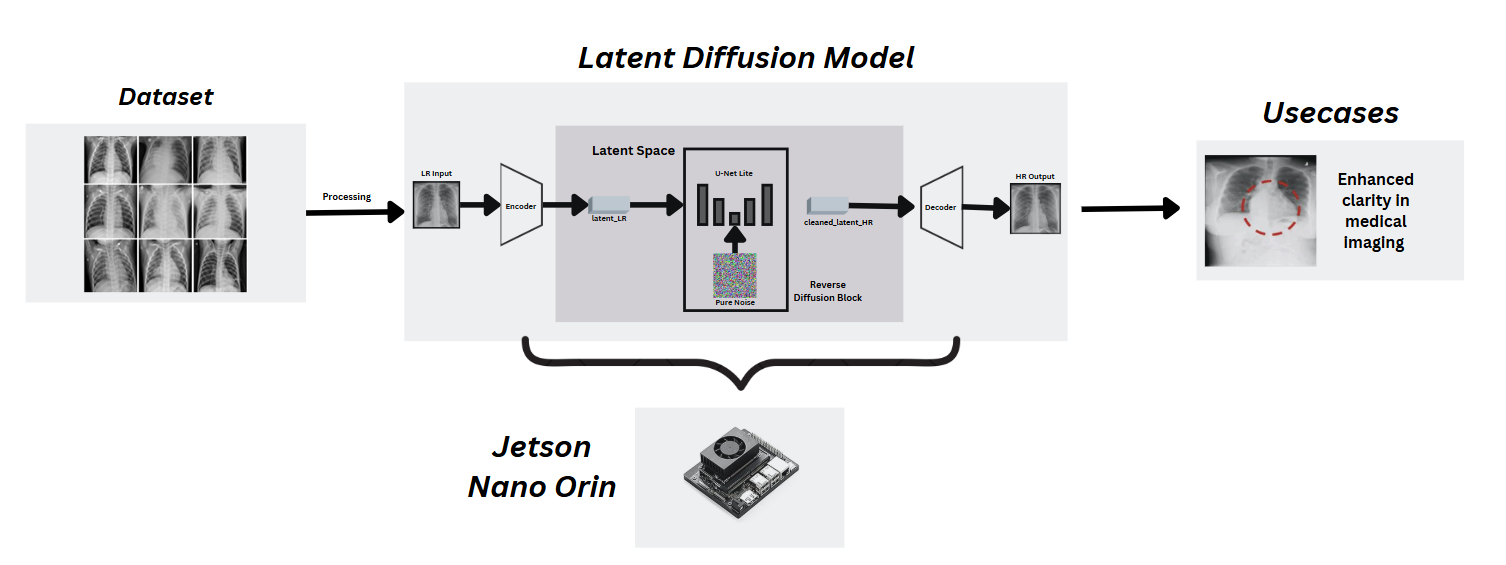
\includegraphics[width=1\textwidth]{Figs/modelmain.png}
\end{center}
\caption{The proposed model.}
\end{figure}

Deep learning is fit for this project as this task does not require interpretability. It will also be able to recover finer details that traditional methods like interpolation-based, reconstruction-based, and learning-based miss. Since our project leverages a large dataset of chest X-ray images, and neural architectures excel at learning complex patterns from extensive data, it deems a good fit for the task. The use of diffusion models, paired with latent space encoders, allows for a flexible and powerful way to upscale LR images. This makes our solution both practically useful and scalable for real-world medical settings, where improving image resolution can directly impact patient diagnosis.

\section{Background And Related Work}

\subsection{A Brief History of Super Resolution (SR)}

Super-resolution (SR) is the task of reconstructing high-resolution (HR) images from low-resolution (LR) counterparts. Early SR methods predominantly involved traditional interpolation techniques like bicubic interpolation, in which weighted averages of surrounding pixels are used to approximate unknown pixel values. It is a general purpose resampling technique used for both upsampling and downsampling. Although computationally efficient, this lacks the ability to capture fine detail and results tend to introduce blur. This is confirmed by the Data Processing Inequality which roughly states that you can not create information that was not present \citep{cover2012elements}. As a result, there have been recent shifts to exploring Deep Neural Network based frameworks as a means to inject learned information from the Neural Networks, into low-resolution images in order to increase resolution in a manner that actually adds informative content. 

\subsection{Evaluation Metrics in Super-Resolution}

Traditional SR approaches typically evaluate quality using metrics such as Peak Signal-to-Noise Ratio (PSNR) and Structural Similarity Index Measure (SSIM) \citep{huynh2008scope, wang2004image}. PSNR quantifies the reconstruction quality based on pixel-wise errors. It is calculated as:

\begin{align}
\text{PSNR} &= 10 \cdot \log_{10} \left( \frac{\text{MAX}^2}{\text{MSE}} \right)
\end{align}

\vspace{-0.5em}
\noindent{where}
\begin{tabbing}
\hspace{2.5em}\=MAX \quad\= Maximum possible pixel value (typically 255 for 8-bit images) \\
\>MSE \> Mean squared error between the original and reconstructed images
\end{tabbing}

\vspace{1em}
SSIM assesses perceptual quality by comparing luminance, contrast, and structure.

\begin{align}
\text{SSIM}(x, y) &= \frac{(2\mu_x \mu_y + C_1)(2\sigma_{xy} + C_2)}{(\mu_x^2 + \mu_y^2 + C_1)(\sigma_x^2 + \sigma_y^2 + C_2)}
\end{align}

\vspace{-0.5em}
\noindent{where}
\begin{tabbing}
\hspace{2.5em}\=$\mu_x$, $\mu_y$ \quad\= Mean intensity of images $x$ and $y$ \\
\>$\sigma_x^2$, $\sigma_y^2$ \> Variance of $x$ and $y$ \\
\>$\sigma_{xy}$ \> Covariance between $x$ and $y$ \\
\>$C_1$, $C_2$ \> Constants to stabilize the division when the denominators are small
\end{tabbing}


PSNR is widely used in papers as it is simple and fast. SSIM, by contrast, tends to favor structural similarity and captures visual structure better than PSNR \citep{wang2004image}.

\subsection{CNN-Based Super-Resolution}

Some of the earliest SR involved the use of CNN based architectures. \citet{dong2015cnn}'s pioneering work, SRCNN, demonstrated CNNs' superiority over traditional methods by achieving substantial improvements in PSNR metrics. These CNN models utilized pixel-wise losses such as L1 and L2 loss, leading to overly smoothed outputs that were not as sharp.

\subsection{GAN-Based Super-Resolution}

In 2017, Generative Adversarial Networks (GANs) showed promising breakthroughs in SR. GANs are a framework that uses two networks in order to generate new data. A generator network generates synthetic data that looks like real data in order to fool a discriminator network who tries to distinguish between real and fake data. The goal is to train the generator to the point where it excels in synthetic data generation by becoming capable enough to fool even the discriminator. SRGAN by \citet{ledig2017gan} significantly improved perceptual quality through adversarial training. This work was further extended by ESRGAN, enhancing GAN training stability and introducing deeper architectures \citep{wang2018esrgan} .
Despite these successes, GAN-based approaches suffer from being notoriously difficult to train. By their very nature, they require delicate balancing between generator and discriminator networks to achieve stable convergence.

\subsection{Pixel-Space UNets and their Limitations}

The U-Net architecture, initially proposed by \citet{ronneberger2015unet}. for biomedical image segmentation, features an encoder-decoder structure. They excel at image-to-image tasks. Its uniqueness lies in the fact that it included skip connections, in which each encoder’s block is saved and passed directly to the corresponding decoder block with the goal of preserving information from earlier layers while still capturing global context via the bottleneck.  U-nets operate in pixel-space, and as a result, end up being memory-intensive and computationally heavy, making them unsuitable for deployment on edge devices and also slow to train.

\subsection{Latent Diffusion Models}

Latent Diffusion Models (LDMs), introduced by \citet{rombach2022latent}, offer computational efficiency by performing diffusion processes in a compressed latent space obtained via a Variational Autoencoder (VAE). Diffusion models iteratively add and remove noise to generate realistic outputs. The key advantage of LDMs lies in reduced computational cost. Latent spaces significantly decrease the input dimensions into the U-Net, thus reducing computation and memory requirements.

LDMs have been effectively employed in state-of-the-art image synthesis frameworks like Stable Diffusion, demonstrating high-quality image generation capabilities \citep{rombach2022latent}. More recently, Edge-SD-SR by \citet{mehdi2025edgesd} showcased latent diffusion-based SR's practicality on mobile and edge devices, dramatically reducing model size and inference latency while preserving quality. Edge-SD-SR achieved impressive results with models as small as ~169M parameters and inference times under 40ms on smartphones, highlighting the potential for real-time applications.

\section{Data Processing}

The NIH ChestX-ray14 dataset that will be used to train this model is a public medical imaging dataset consisting of 112,120 chest X-ray images (1024 × 1024 pixels) from 30,805 unique patients. To manage storage and training time, three image archive batches (approximately 30,000 images) will be selected. These images will be filtered for PA (posteroanterior) view X-rays because they are the clinical standard and offer minimal distortion compared to AP views. Corrupted and non-standard images will also be discarded. Approximately 10,000–15,000 high-resolution X-rays will remain for training, validation, and testing.

The following preprocessing methods will be used by the team as needed:

\begin{enumerate}
    \item \textbf{Generating HR and LR Image Pairs:} Due to memory limitations and hardware constraints, the original 1024² images will be resized to a resolution of 256 × 256 pixels using bicubic interpolation (OpenCV’s \texttt{INTER\_CUBIC}). These resized images will serve as the ground-truth high-resolution (HR) set. A further downsampled copy of each 256² image, also using bicubic interpolation, will be generated at 64 × 64 pixels to simulate low-resolution (LR) inputs for the super-resolution task. Matching LR and HR images will be stored as pairs with identical filenames in two separate folders (\texttt{HR\_256} and \texttt{LR\_64}) for ease of access.

    \item \textbf{Data Loading and Tensor Conversion:} After disk pre-processing, each LR-HR image pair will be loaded. PNG images will first be loaded from disk into NumPy arrays as 8-bit integers with pixel values ranging from 0 to 255. These arrays will be converted into PyTorch tensors of datatype float32 and normalized by dividing by 255.0, scaling pixel values into the range [0.0, 1.0]. We will further standardize these tensors by shifting and scaling them to a range of [-1, 1], which is standard in latent-diffusion-based models to accelerate training convergence.

    \item \textbf{Data Augmentation:} To improve model generalization, identical random horizontal flips, ± 15° rotations, and slight brightness jitter will be applied consistently to each LR-HR image pair using a shared pipeline from \texttt{torchvision.transforms}. This approach ensures both images in a pair maintain perfect alignment after augmentation.

    \item \textbf{Mini-Batch Assembly:} Finally, a PyTorch DataLoader will assemble mini-batches consisting of tensors shaped \texttt{(B × 1 × 64 × 64)} for LR images and \texttt{(B × 1 × 256 × 256)} for HR images, feeding them directly into the diffusion-based super-resolution model during training and evaluation.

    \item \textbf{Dataset Splitting:} The processed dataset will be divided into training, validation, and testing subsets with a split of 70\% training, 20\% validation, and 10\% testing.
\end{enumerate}


\section{Architecture}

The project aims to perform SR via a latent diffusion based architecture. It has critical simplifications to enable edge deployment and efficient training. The system will consist of a pretrained Variational Autoencoder, a custom denoising U-Net lite which will be implemented, and a diffusion noise scheduler. The VAE and diffusion noise scheduler will be borrowed from Hugging Face open source library.

\begin{figure}[h]
\begin{center}
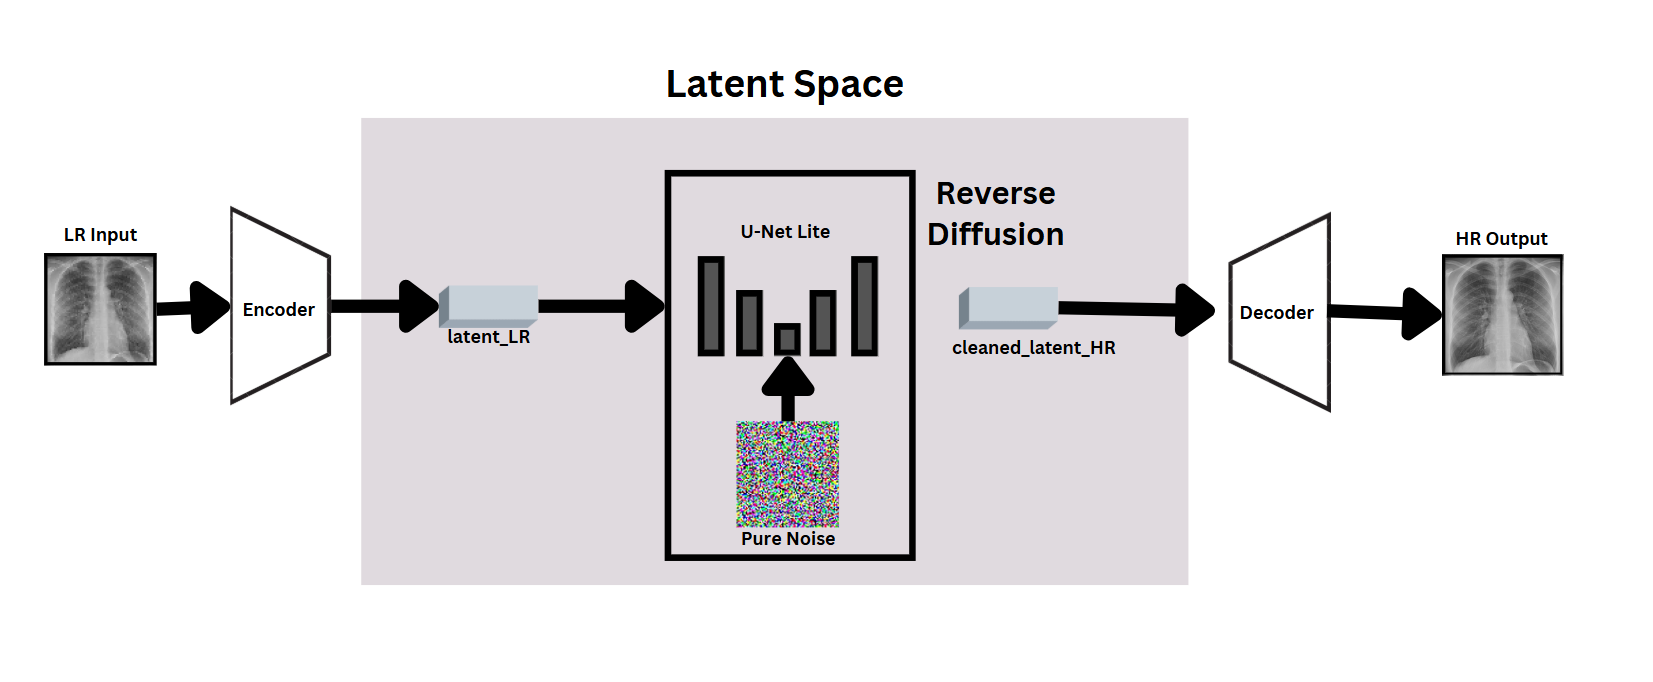
\includegraphics[width=0.9\textwidth]{Figs/model.png}
\end{center}
\caption{Proposed model architecture.}
\end{figure}

\subsection{Training Pipeline}

During training, each high-resolution (HR) and low-resolution (LR) image pair is first encoded by a frozen Variational Autoencoder (VAE) encoder into latent representations (\texttt{latent\_HR} and \texttt{latent\_LR}). The HR latent then undergoes forward diffusion, in which Gaussian noise of intensity t (referred to commonly as the timestep), is added according to a scheduler in a stochastic manner, yielding a noisy latent (\texttt{noisy\_latent\_HR}). The custom UNet-Lite model takes this noisy latent, along with the LR latent and timestep, to predict the exact noise that was added. The training objective is to minimize the mean squared error (MSE) between the predicted noise and the true added noise, allowing the UNet-Lite model to learn effective denoising patterns at various noise levels.

\subsection{Inference Pipeline}

At inference (deployment on Jetson Nano), only the LR image is available, which is first encoded by the frozen VAE encoder into \texttt{latent\_LR}. The inference process starts from pure Gaussian noise (\texttt{latent\_N}), which is iteratively denoised through a reverse diffusion loop using the trained UNet-Lite model. At each reverse diffusion step, the model predicts and removes noise, conditioned on \texttt{latent\_LR}, gradually refining the latent representation. After completing 20-30 reverse diffusion steps, the final clean latent is decoded by the frozen VAE decoder into the high-resolution, super-resolved output image.

\subsection{Edge AI Deployment}

After training, the custom UNet-Lite model and VAE decoder will be exported from PyTorch into ONNX format and quantized to INT8 precision using NVIDIA’s TensorRT, significantly reducing inference latency and memory usage. The optimized INT8 models will be deployed on a Jetson Nano development kit. During inference on the Jetson device, a lightweight Python interface will accept 64×64 LR images, run the entire latent diffusion super-resolution pipeline, and display the generated 256×256 super-resolved outputs along with inference times.

\section{Baseline Model}

The model’s outputs will be compared to a baseline such as bicubic upsampling, where the LR image will be taken as input and resized to a HR image via bicubic. Then, PSNR/SSIM will be computed against ground truth and a baseline number will be set up. Ideally the model should exceed or at least match  the baseline number with better perceptual quality.

\section{Ethical Considerations}

While this project aims to improve diagnostic support by enhancing low-resolution chest X-ray images through latent diffusion, several ethical considerations and limitations must be addressed.

\subsubsection{Data and Labeling Limitations}

The dataset that will be used in this project consists of chest X-rays images with labels extracted from radiology reports via Natural Language Processing (NLP). Although the labelling method achieves over 90\% accuracy, they are not manually verified by radiologists. This introduces labeling noise and some positive findings may actually be false or ambiguous in the image itself \citep{olatunji2019caveats}.


\subsection{Bias and Generalizability}

Public datasets, like the one being used for this project usually lack demographic diversity, which risks bias and reduced performance on underrepresented populations \citep{Galanty2024BEAMRAD}.

\subsection{Model and Practical Constraints}

The diffusion-based architecture relies on generative modeling in a latent space, which may introduce hallucinated details not present in the original scan. While the UNet-Lite reduces complexity for edge deployment, it may limit the model’s ability to capture subtle clinical features. Additionally, using a pretrained VAE not tailored to medical images may lead to domain mismatch.

\subsection{Clinical Risks}

Super-resolution can enhance clarity but may introduce artifacts or hallucinations. These enhancements must not be mistaken for real anatomical features, as they could mislead diagnoses if not carefully validated \citep{Shin2024SuperResolution}.


Overall, while promising, this system should be used with caution and further validated for safe, fair clinical use.

\section{Project Plan}

\subsection{Communication}

Communication primarily occurs through Discord for day-to-day coordination, while shared Google Drive is used to store and organize documents. GitHub manages code contributions, and ClickUp is used to plan tasks and track progress with Gantt charts. To avoid code conflicts, the team uses feature branches and pull requests in GitHub, ensuring changes are reviewed and merged systematically.

To maintain effective collaboration, the team has scheduled regular weekly meetings on Thursdays at 6:00 PM and Saturdays at 12:00 PM. While in-person attendance is preferred, team members who are unavailable can join virtually via Google Meet.

\begin{table}[h!]
\captionsetup{justification=centering}
\caption{Platforms used for team collaboration and project execution.}
\label{platforms-table}
\centering
\renewcommand{\arraystretch}{1.5}
\setlength{\tabcolsep}{8pt}
\begin{tabularx}{\textwidth}{@{} >{\raggedright\arraybackslash}p{3cm} >{\raggedright\arraybackslash}p{3cm} >{\raggedright\arraybackslash}X @{}}
\toprule
\multicolumn{1}{c}{\textbf{Platform}} & 
\multicolumn{1}{c}{\textbf{Purpose}} & 
\multicolumn{1}{c}{\textbf{Description}} \\
\midrule
Discord & Main communication & Used for daily team communication, quick updates, and coordination. \\
\addlinespace
Shared Google Drive & File storage \& collaboration & Central location for organizing and sharing documents, slides, and resources. \\
\addlinespace
GitHub & Code collaboration & Repository for version control, code sharing, and collaborative development. \\
\addlinespace
Google Meet & Virtual meetings & Used for remote team meetings, discussions, and check-ins. \\
\addlinespace
ClickUp & Scheduling and Project Management & To plan weekly meetings, set deadlines, assign tasks, and coordinate teamwork sessions using Gantt charts. \\
\bottomrule
\end{tabularx}
\end{table}

\subsection{Task division}

The team has divided the project into clear components aligned with the architecture stages: data preparation, latent encoding, forward diffusion, denoising (training), reverse diffusion (inference), decoding, and deployment. Each team member is assigned responsibility for specific tasks within these stages, with deadlines set to ensure steady progress and timely completion. 

\begin{table}[h]
\caption{Team member responsibilities and specialization areas.}
\label{team-table}
\begin{center}
\begin{tabular}{lll}
\toprule
\multicolumn{1}{c}{\bf Member} &
\multicolumn{1}{c}{\bf Primary Focus} &
\multicolumn{1}{c}{\bf Secondary Focus} \\
\midrule
A: Ayushi Agrawal   & Data Processing \& Evaluation     & Deployment testing, slide design \\
\addlinespace
B: Saaim Raad       & Model Architecture                & Dataset integration, training \& docs \\
\addlinespace
C: Md Nazmus Saad   & Diffusion \& Deployment           & Model training \& evaluation metrics \\
\addlinespace
D: Pakhi Gupta      & Documentation \& UI               & Data pairing, augmentation, visualization \\
\bottomrule
\end{tabular}
\end{center}
\end{table}

\newpage
\begin{table}[h!]
\captionsetup{justification=centering}
\caption{Project task breakdown and responsible team members.}
\label{task-table}
\centering
\renewcommand{\arraystretch}{1} 
\setlength{\tabcolsep}{6pt}       % reduce column padding a bit
\begin{tabularx}{\textwidth}{>{\raggedright\arraybackslash}X >{\centering\arraybackslash}m{1cm} >{\centering\arraybackslash}m{1.5cm} >{\raggedright\arraybackslash}m{7cm}}
\textbf{Task} & \textbf{Member} & \textbf{Due} & \textbf{Description} \\
\midrule
Download and extract data & A, D & June 17 & Prepare base image folder \\
\addlinespace
Filter images from metadata & A, D & June 17 & Manually select relevant data \\
\addlinespace
Resize and create HR–LR pairs & A, D & June 17 & Downsample to 64×64 (LR), resize to 256×256 (HR), and pair for training \\
\addlinespace
Implement PyTorch Dataset class & D, B & June 22 & Code loading logic with augmentations; support LR–HR image pairing \\
\addlinespace
Implement VAE encoder/decoder & B, C & June 24 & Design latent-space VAE with encoder, decoder, and reparameterization trick \\
\addlinespace
Build UNet-Lite architecture & B, A & July 2 & Create U-Net with skip connections, tuned for latent noise prediction \\
\addlinespace
Implement diffusion scheduler & C, B & July 5 & Code forward and reverse noise processes, timestep handling, and $\beta$ scheduler \\
\addlinespace
Train initial model & C, B & July 9 & Train with 10k steps, log loss, PSNR, and LPIPS on validation split \\
\addlinespace
Test model using evaluation metrics & A, C & July 10 & Add PSNR, LPIPS, FID, and validation logging for model evaluation \\
\addlinespace
Draft progress report & All & July 11 & Each member writes a section; final draft compiled and submitted as a group \\
\addlinespace
Export model to ONNX & C, B & July 20 & Convert trained model to ONNX format, validate output shape and consistency \\
\addlinespace
Quantize with TensorRT (INT8) & C, B & July 25 & Use TensorRT to quantize model and benchmark latency on Jetson \\
\addlinespace
Create Streamlit/Jetson demo & C, A & July 29 & Build interface to show before/after on edge device \\
\addlinespace
Generate final poster/slides & D, A & Aug 10 & Design final visuals, graphs, and flow diagrams for presentation \\
\bottomrule
\end{tabularx}
\end{table}

An example of task division using ClickUp Gantt charts for this project is shown below, illustrating how tasks are broken down and scheduled over time.

\begin{figure}[h]
\begin{center}
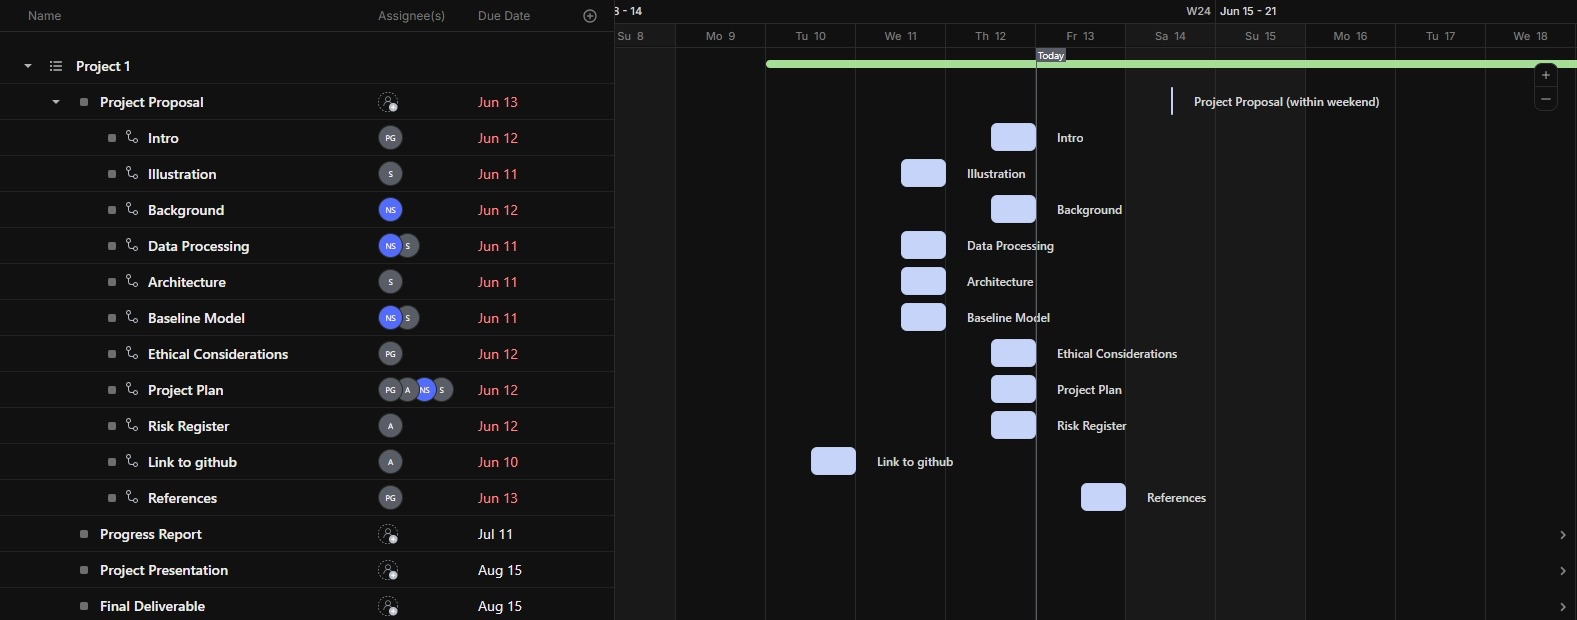
\includegraphics[width=1\textwidth]{Figs/gantt.jpg}
\end{center}
\caption{Gantt Chart using ClickUp.}
\end{figure} 

\section{Risk Register}

Both technical and collaborative issues may arise during the course of the project. Some key risks are outlined in the table below. The impact of an event and its likelihood are scored on a scale of 1 to 5. The risk is calculated as the product of these two metrics.

\newpage

\renewcommand{\arraystretch}{1.4}
\definecolor{risklow}{RGB}{255,255,153}    % Yellow
\definecolor{riskmed}{RGB}{255,204,102}    % Orange
\definecolor{riskhigh}{RGB}{255,102,102}   % Red

\begin{table}[h!]
\centering
\caption{Risk register with impact, likelihood, and mitigation strategies.}
\renewcommand{\arraystretch}{1.2} % tighter row spacing
\setlength{\tabcolsep}{6pt}       % tighter column padding
\begin{tabularx}{\textwidth}{|>{\raggedright\arraybackslash}X|>{\raggedright\arraybackslash}X|>{\centering\arraybackslash}p{0.5cm}|>{\raggedright\arraybackslash}p{6cm}|}
\hline
\textbf{Event, Impact} & \textbf{Likelihood} & \textbf{Risk} & \textbf{Mitigation Strategy} \\
\hline

Team member drops out or becomes unresponsive. \textbf{Score: 3} &
Unlikely; members need the skills acquired from this course. \textbf{Score: 1} &
\cellcolor{risklow}3 &
(1) Maintain clear and consistent documentation and internal progress reports. (2) Write well-structured and commented code. (3) Reevaluate team goal and redistribute tasks. \\
\hline

Model training takes significantly longer than expected. \textbf{Score: 4} &
Likely; we are attempting to train on large datasets without extensive resources. \textbf{Score: 5} &
\cellcolor{riskhigh}12 &
(1) Start with smaller datasets or lower resolution. (2) Consider transfer learning. (3) Parallelize where possible. (4) Monitor training time early and adjust if needed. \\
\hline

Model exceeds latency or memory limits on edge device. \textbf{Score: 5} &
Possible; although device has 8GB RAM memory which should suffice. \textbf{Score: 4} &
\cellcolor{riskhigh}10 &
(1) Quantize aggressively. (2) Profile on-device early. (3) Adjust architecture (e.g., smaller U-Net). (4) Fall back to simpler SR model if absolutely needed (i.e., CNN-based or GAN). \\
\hline

Quantization severely degrades SR output quality. \textbf{Score: 3} &
Likely; Super-resolution is a fine-grained image generation task, where 8-bit quantization can easily blur or destroy details. \textbf{Score: 5} &
\cellcolor{riskmed}9 &
(1) Retrain model while simulating quantization from the start. (2) Use half precision (FP16 instead of INT8). \\
\hline

Generated images contain unrealistic textures or artifacts. \textbf{Score: 3} &
Likely; models are unpredictable and outputs may be unexpected. \textbf{Score: 5} &
\cellcolor{riskmed}9 &
(1) Increase UNet size. (2) Ensure diverse training data. (3) Tune noise schedule and regularization. (4) Visually monitor outputs during training. \\
\hline

Team falls behind due to unclear division of work or miscommunication. \textbf{Score: 3} &
Unlikely; project plan is detailed and individually assigned. \textbf{Score: 2} &
\cellcolor{risklow}3 &
(1) Assign clear roles early. (2) Hold weekly sync-ups. (3) Use a shared Notion/GitHub board. (4) Create a communication protocol (e.g., Discord updates, weekly deliverables). \\
\hline

Deployment tools (e.g., TensorRT or ONNX) are incompatible or unstable. &
Moderate; ONNX conversion for diffusion models can be tricky. \textbf{Score: 3} &
\cellcolor{riskmed}9 &
(1) Test the pipeline early. (2) Document known compatibility issues. (3) Be ready to adjust pipeline (e.g., simplify model or use different tools). (4) Be prepared to try Snapdragon (Qualcomm interface). \\
\hline
\end{tabularx}
\end{table}

\section{Link to GitHub Repository}

GitHub will be used to store and collaborate on code for this project. The link to the repository is: \url{https://github.com/petrichor-2/image-upscaler}

\clearpage

\label{last_page}

\bibliography{APS360_ref}
\bibliographystyle{iclr2022_conference}

\end{document}
